%-----------------------------------LICENSE------------------------------------%
%   This file is part of tikz_figures.                                         %
%                                                                              %
%   tikz_figures is free software: you can redistribute it and/or              %
%   modify it it under the terms of the GNU General Public License as          %
%   published by the Free Software Foundation, either version 3 of the         %
%   License, or (at your option) any later version.                            %
%                                                                              %
%   tikz_figures is distributed in the hope that it will be useful,            %
%   but WITHOUT ANY WARRANTY; without even the implied warranty of             %
%   MERCHANTABILITY or FITNESS FOR A PARTICULAR PURPOSE.  See the              %
%   GNU General Public License for more details.                               %
%                                                                              %
%   You should have received a copy of the GNU General Public License along    %
%   with tikz_figures.  If not, see <https://www.gnu.org/licenses/>.           %
%------------------------------------------------------------------------------%

% Use the standalone class for displaying the tikz image on a small PDF.
\documentclass[crop, tikz]{standalone}

% Import the tikz package to use for the drawing.
\usepackage{tikz}

% Begin the document.
\begin{document}

    % Begin the drawing.
    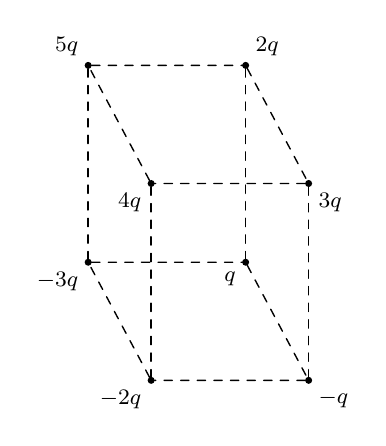
\begin{tikzpicture}[%
        line width = 0.5pt,
        line cap = round,
        font = \footnotesize
    ]

        % Locations of all of the points.
        \begin{scope}[%
            every node/.style = {
                circle,
                fill = black,
                draw = black,
                inner sep = 0pt,
                minimum size = 2pt
            }
        ]
            \node (a) at (0,0) {};
            \node (b) at (2,0) {};
            \node (c) at (2.8,-1.5) {};
            \node (d) at (0.8,-1.5) {};
            \node (e) at (0,-2.5) {};
            \node (f) at (2,-2.5) {};
            \node (g) at (2.8,-4) {};
            \node (h) at (0.8,-4) {};
        \end{scope}

        % Label the charges at the points.
        \node at (a) [above left] {$5q$};
        \node at (b) [above right] {$2q$};
        \node at (c) [below right] {$3q$};
        \node at (d) [below left] {$4q$};
        \node at (e) [below left] {$-3q$};
        \node at (f) [below left] {$q$};
        \node at (g) [below right] {$-q$};
        \node at (h) [below left] {$-2q$};

        % Dashed lines connecting the points.
        \draw[dashed] (a) to (2,0) (b) to (c) to (d) to (a);
        \draw[dashed] (e) to (f) to (g) to (h) to (e);
        \draw[dashed] (a) to (e);
        \draw[dashed] (b) to (f);
        \draw[dashed] (c) to (g);
        \draw[dashed] (d) to (h);
    \end{tikzpicture}
\end{document}
